\section{Imperial College Press Release, 24 August 2012}


\textbf{Imperial explorers find Slovenia’s longest caves}


\textit{www.imperial.ac.uk/news/113166}

\tweet{12:12PM Aug 17, 2012}{Congratulations to Imperial College Caving Society who have discovered the longest cave in Slovenia. \mininame{@icunion}}

The longest cave in Slovenia has been discovered by students and postdocs from Imperial during their summer caving expedition.

“Imagine looking back at your footprints in the sand of a cave floor and knowing those are the first footprints to ever disturb that sand, you are the first people to ever reach that place.” That, Aeronautics student Clare Tan explains, was one of the most exciting moments in her exploration of the caving system under the Slovenian mountain of Tolminski Migovec.

Members of the Imperial College Caving Club have been working with enthusiasts from Caving Section of the Tolmin Alpine Club, exploring two caving systems, Migovec and Vrtnarija, since 1994. In that time over 80 students from Imperial have been involved, delving further in to the winding dark passages with each expedition.

\begin{marginfigure}
\checkoddpage \ifoddpage \forcerectofloat \else \forceversofloat \fi
\centering
 \frame{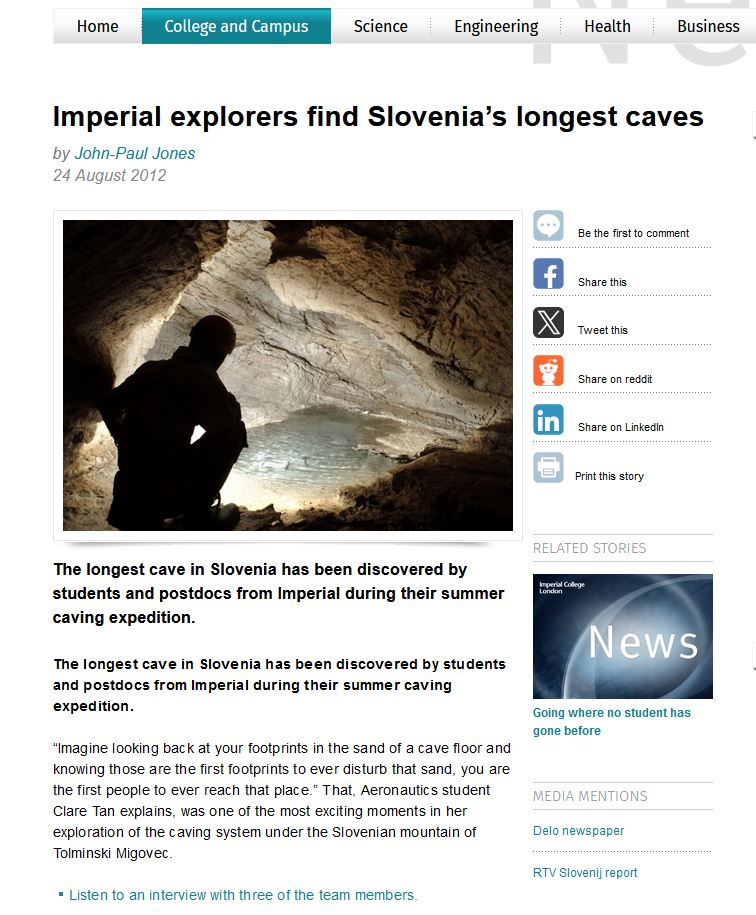
\includegraphics[width=\linewidth]{2012/press_release/pressreleasescreenshot.JPG}} 
 \caption{The Imperial College press release.}
 \label{connection press release screenshot}
\end{marginfigure}

The breakthrough on this year’s trip was the discovery of passages connecting the two systems and proving they are in fact part of one colossal cave system which at 24.9 km long and 975m deep, has displaced Postojna Cave as the country’s longest.  The team’s activities captured the attention of the Slovenian media, with pieces appearing on RTV Slovenij, Slovenia’s national public broadcasting station and in Delo, the largest national daily newspaper.

The team plan to return to the caves to trek down more unvisited passages and explore potential research opportunities, looking at what rock samples from deep in the caves can tell us about climate change, as well as how rain is channelled down through the mountain caves to be the area’s chief water source.

The expedition was supported by Imperial College Union and the Ghar Parau Foundation.

\name {John-Paul Jones, Communications and Public Affairs}


Article text (excluding photos or graphics) available under an Attribution-NonCommercial-ShareAlike Creative Commons license.

Photos and graphics subject to third party copyright used with permission or © Imperial College London.



%This summer Imperial College Caving Club discovered the longest cave in Slovenia during their Sledi Vetra 2012 expedition.

%The Imperial cavers have organised joint expeditions with the local Slovene club (JSPDT) to the mountain of \passage[mountain]{Tolminski Migovec} since 1994, with more than 80 Imperial students having contributed to the discovery. Every year they explored deeper and further into the mountain, the main discoveries being two large and deep cave systems (\passage{System Migovec} and \passage{System Vrtnarija}), both notable caves in their own right. A further 2000 m of cave passage was discovered this summer, leading to the connection of these two cave systems at a depth of 650 m.

%The combined cave system is 24.9 km long and 975 m deep. The deepest point was found this summer where the cave passage leads down into an extensive crystal clear flooded section. The vast majority of such long cave systems in the world are shallow and warm, which greatly eases their exploration. The \passage{Migovec} caves are deep, extremely vertical and cold, requiring a high degree of technical skill and physical endurance.

%\passage[mountain]{Tolminski Migovec} is on the edge of a major thrust complex, the Slatna overthrust, with steeply dipping faults cutting and offsetting the thrusts. A complex series of faults and folds have led to extremely complicated cave formation in the Triassic limestone, the computer model of the mountain’s cave passage looking like a piece of shattered glass. Understanding the hydrology of the mountain is significant as it is the watershed of the Adriatic and Black Seas.

%Deep exploration is made possible by the team remaining underground for 3-4 days at a time, sleeping over 600 metres below the surface of the mountain. As well as the physical challenge, they have had to innovate in developing new methods and techniques – for instance in climbing with a lightweight cordless drill adapted for caving and fitted with external batteries recharged by solar power.

%The connection of these systems, and the discovery of the longest cave in Slovenia has been the major effort and activity of the Imperial cavers for the last five years. But the exploration of \passage{Migovec} is certainly not over – every new passage reveals a new place within the mountain, and no one can possibly tell what will lie around the next corner.

%\name{Jarvist Moore Frost}

\newpage

To put into words how much the connection means to the people who have spent years (even decades!) dedicating their free time to this exploration project is difficult. But Clewin (first expedition 1997) put it beautifully: "Everybody has a made a contribution, from surveying hundreds of meters of horizontal passages to pushing ridiculously tight rifts or squalid muddy dead ends to feeding hungry cavers in the bivvy."
\name{Jarvist Frost}



    \begin{figure*}[t!]
\checkoddpage \ifoddpage \forcerectofloat \else \forceversofloat \fi
\centering
\begin{subfigure}[t]{0.49\textwidth}
\centering
\frame{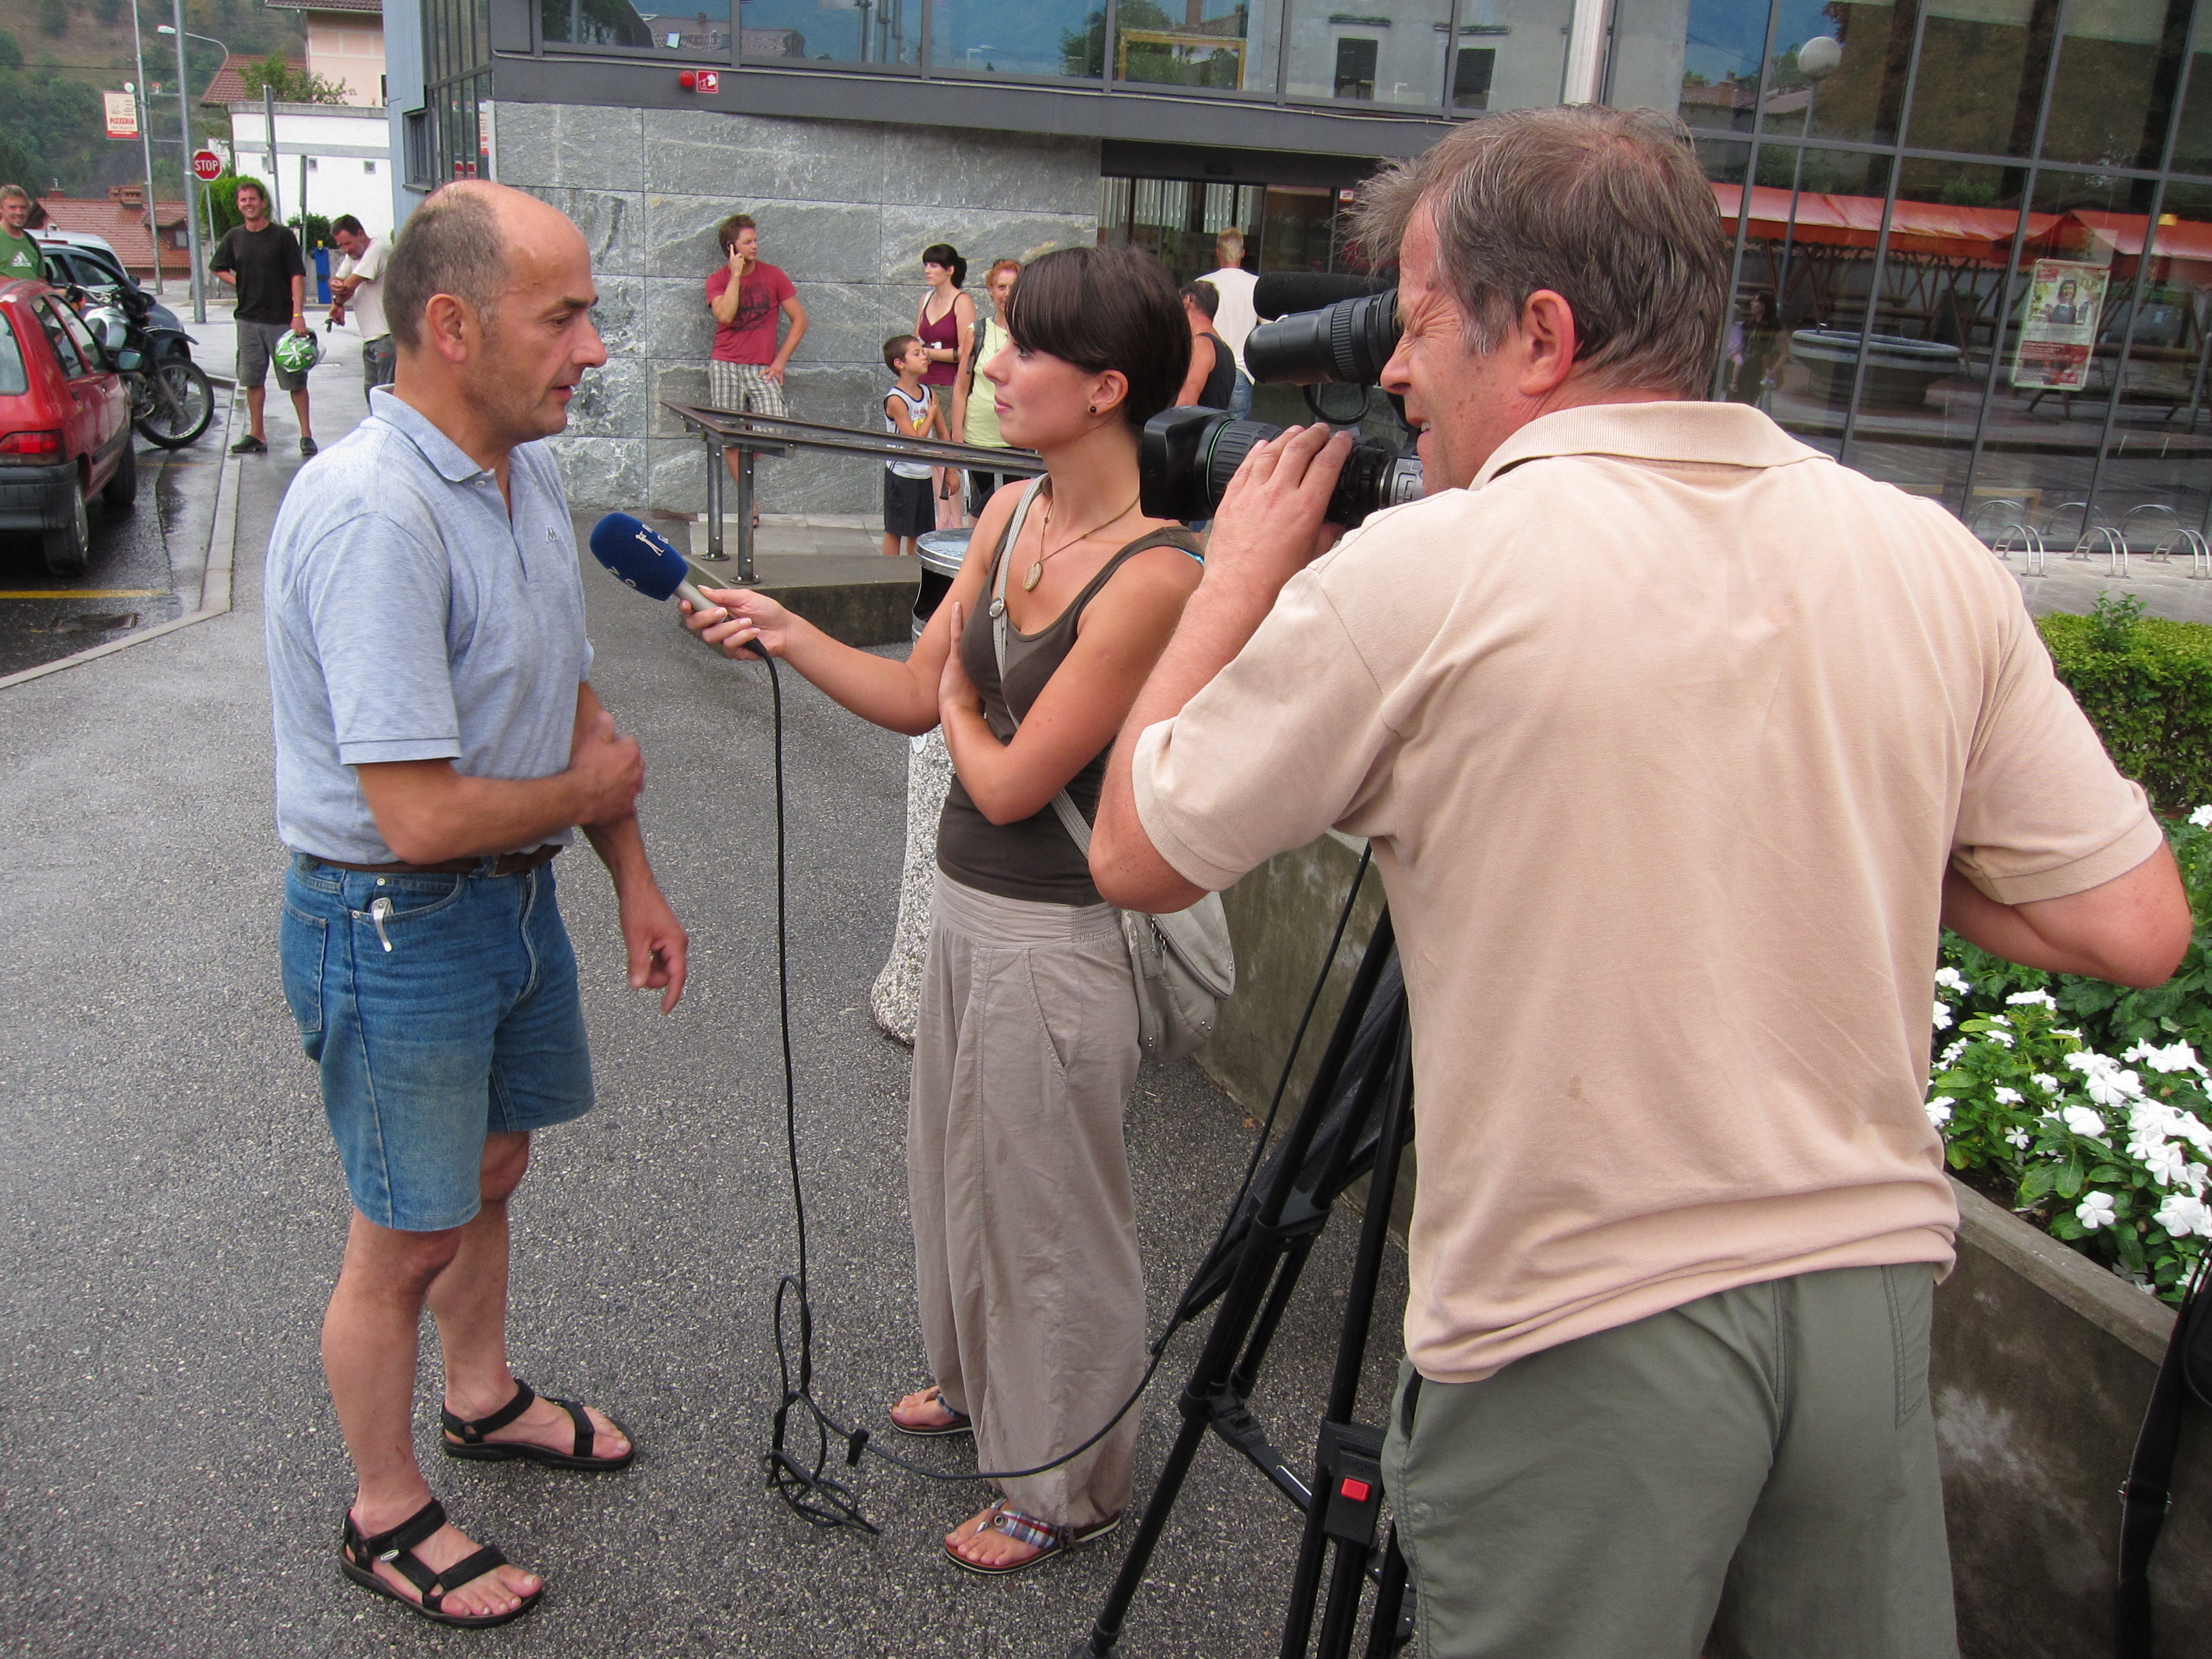
\includegraphics[width=\linewidth]{2012/press_release/2012-08-16-1556-JanaCarga-419--orig.jpg}}
 \caption{}\label{fratnik interview}
\end{subfigure}
    \hfill
    \begin{subfigure}[t]{0.49\textwidth}
        \centering
        \frame{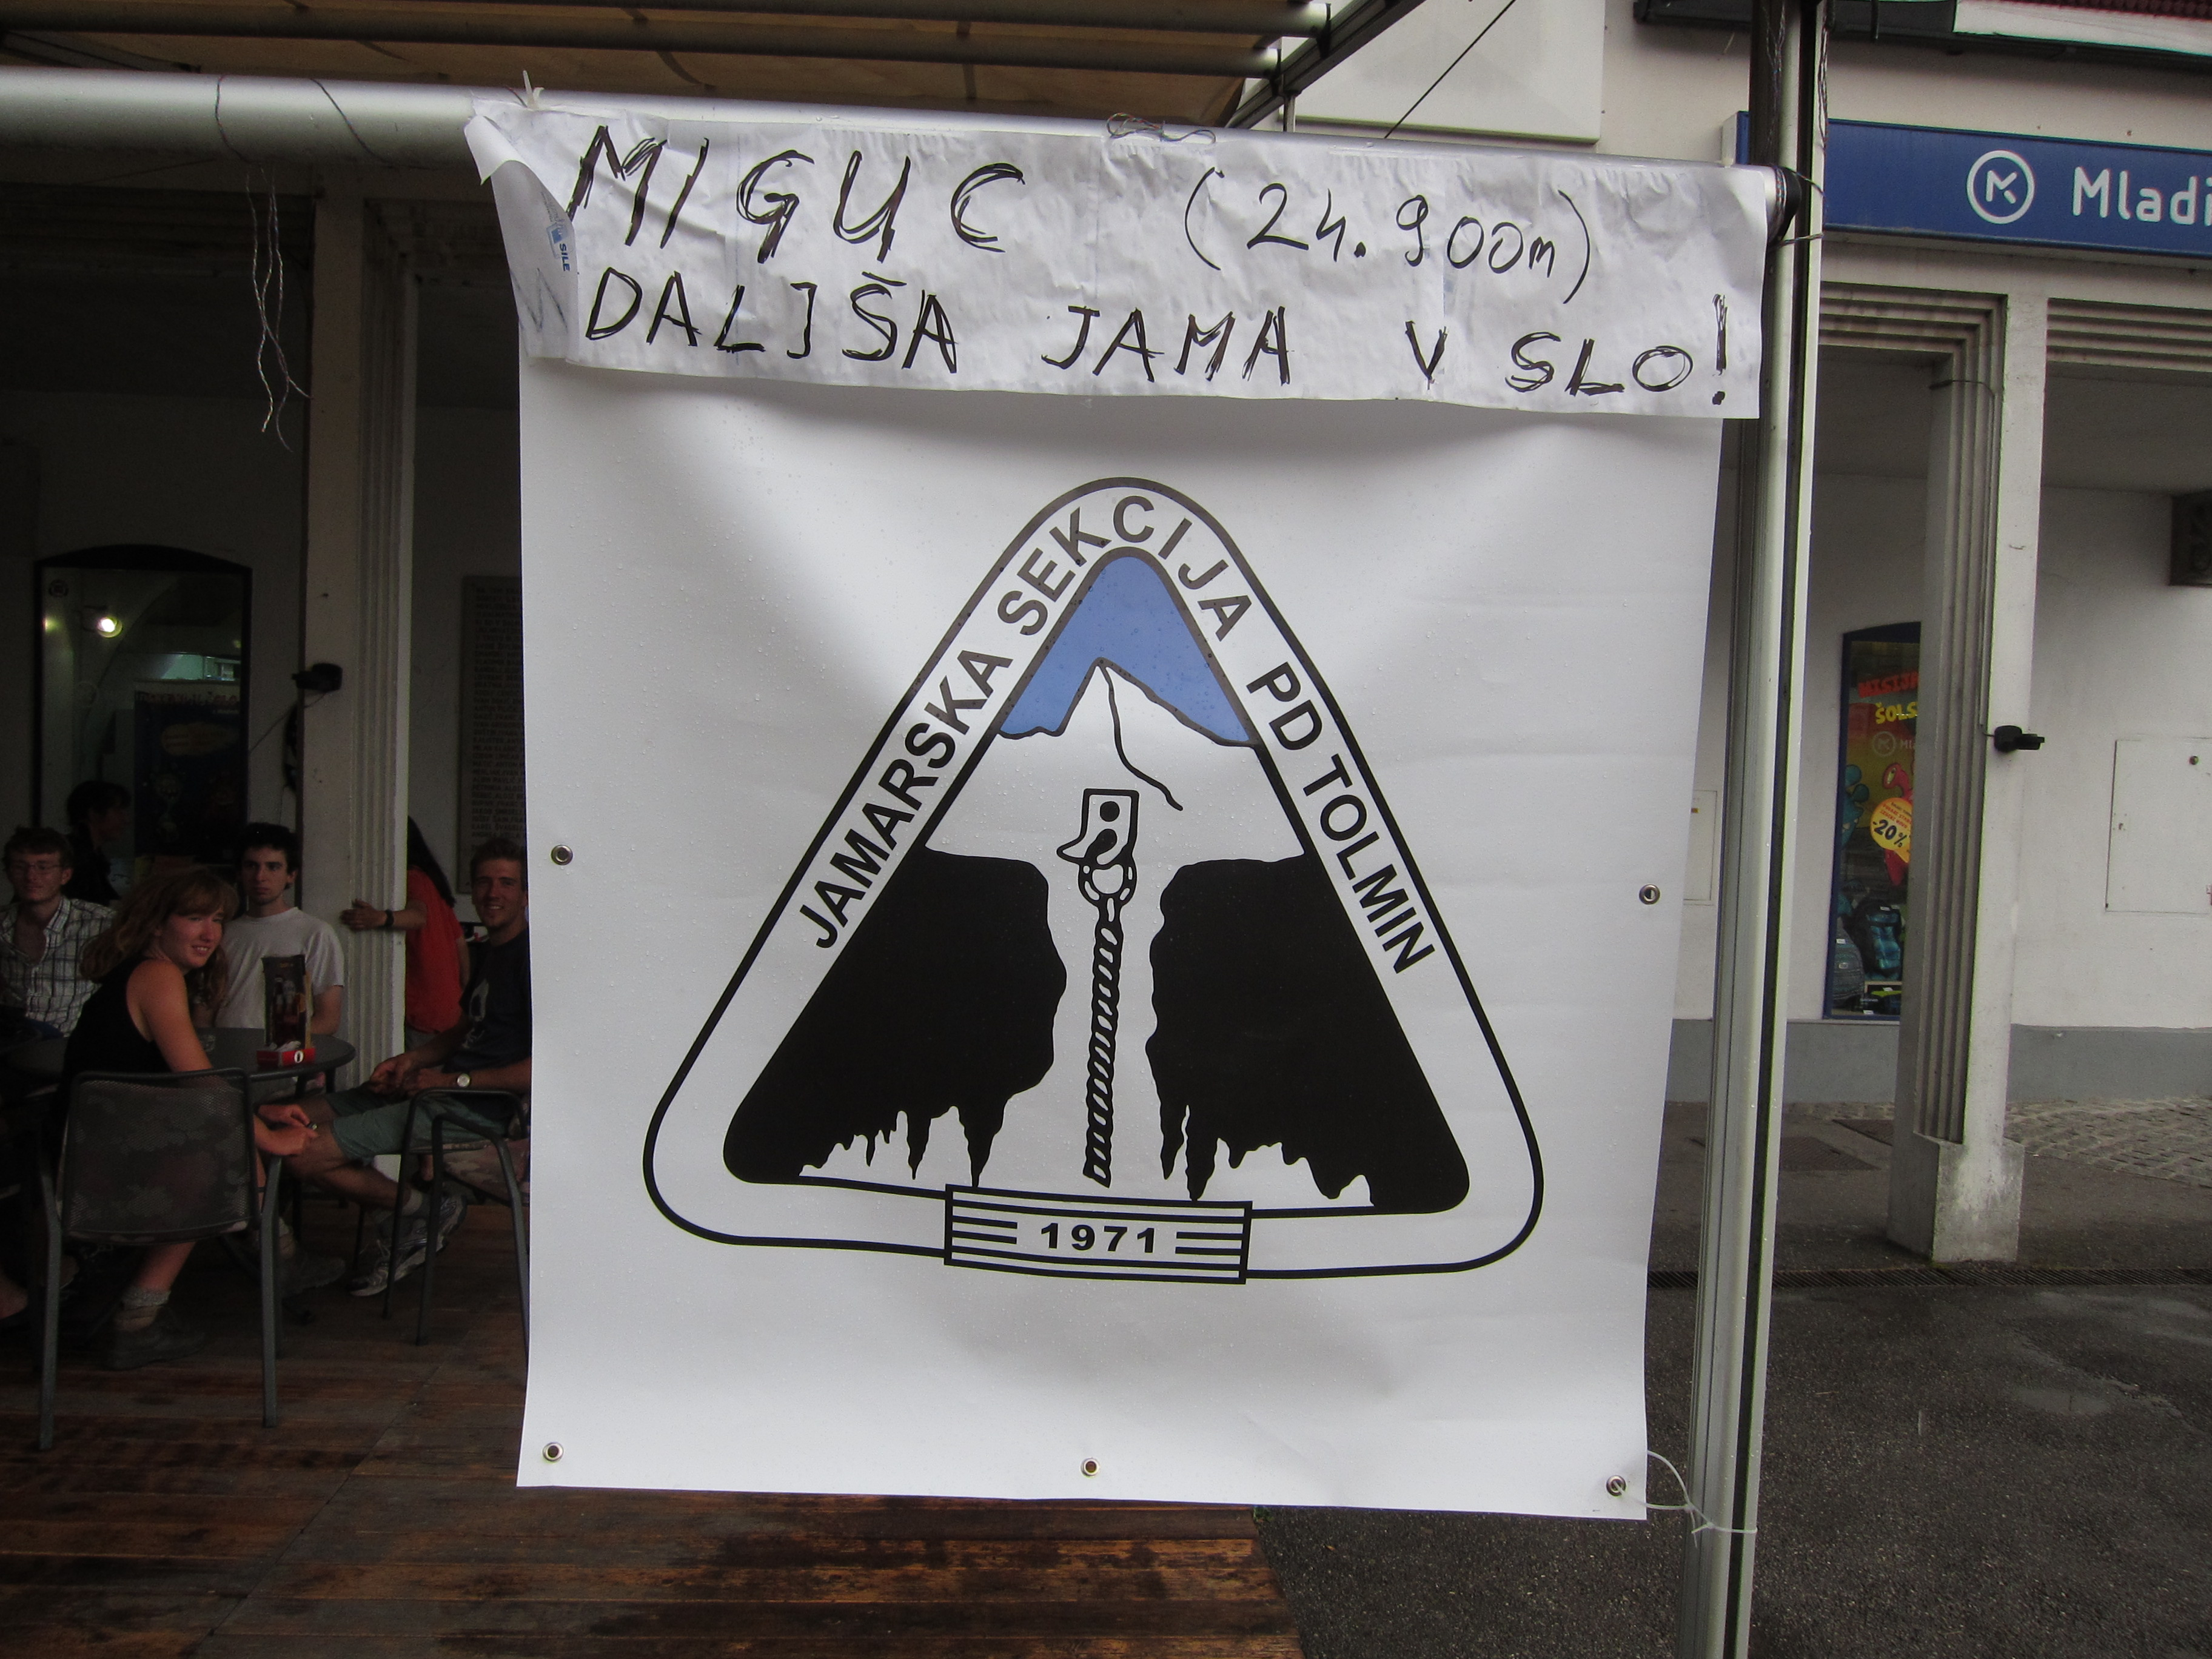
\includegraphics[width=\linewidth]{2012/press_release/2012-08-16-1602-JanaCarga-421--orig.jpg}} 
        \caption{} \label{jama v slov}
    \end{subfigure}
    
    \vspace{0.3cm}
    \begin{subfigure}[t]{\textwidth}
    \centering
        \frame{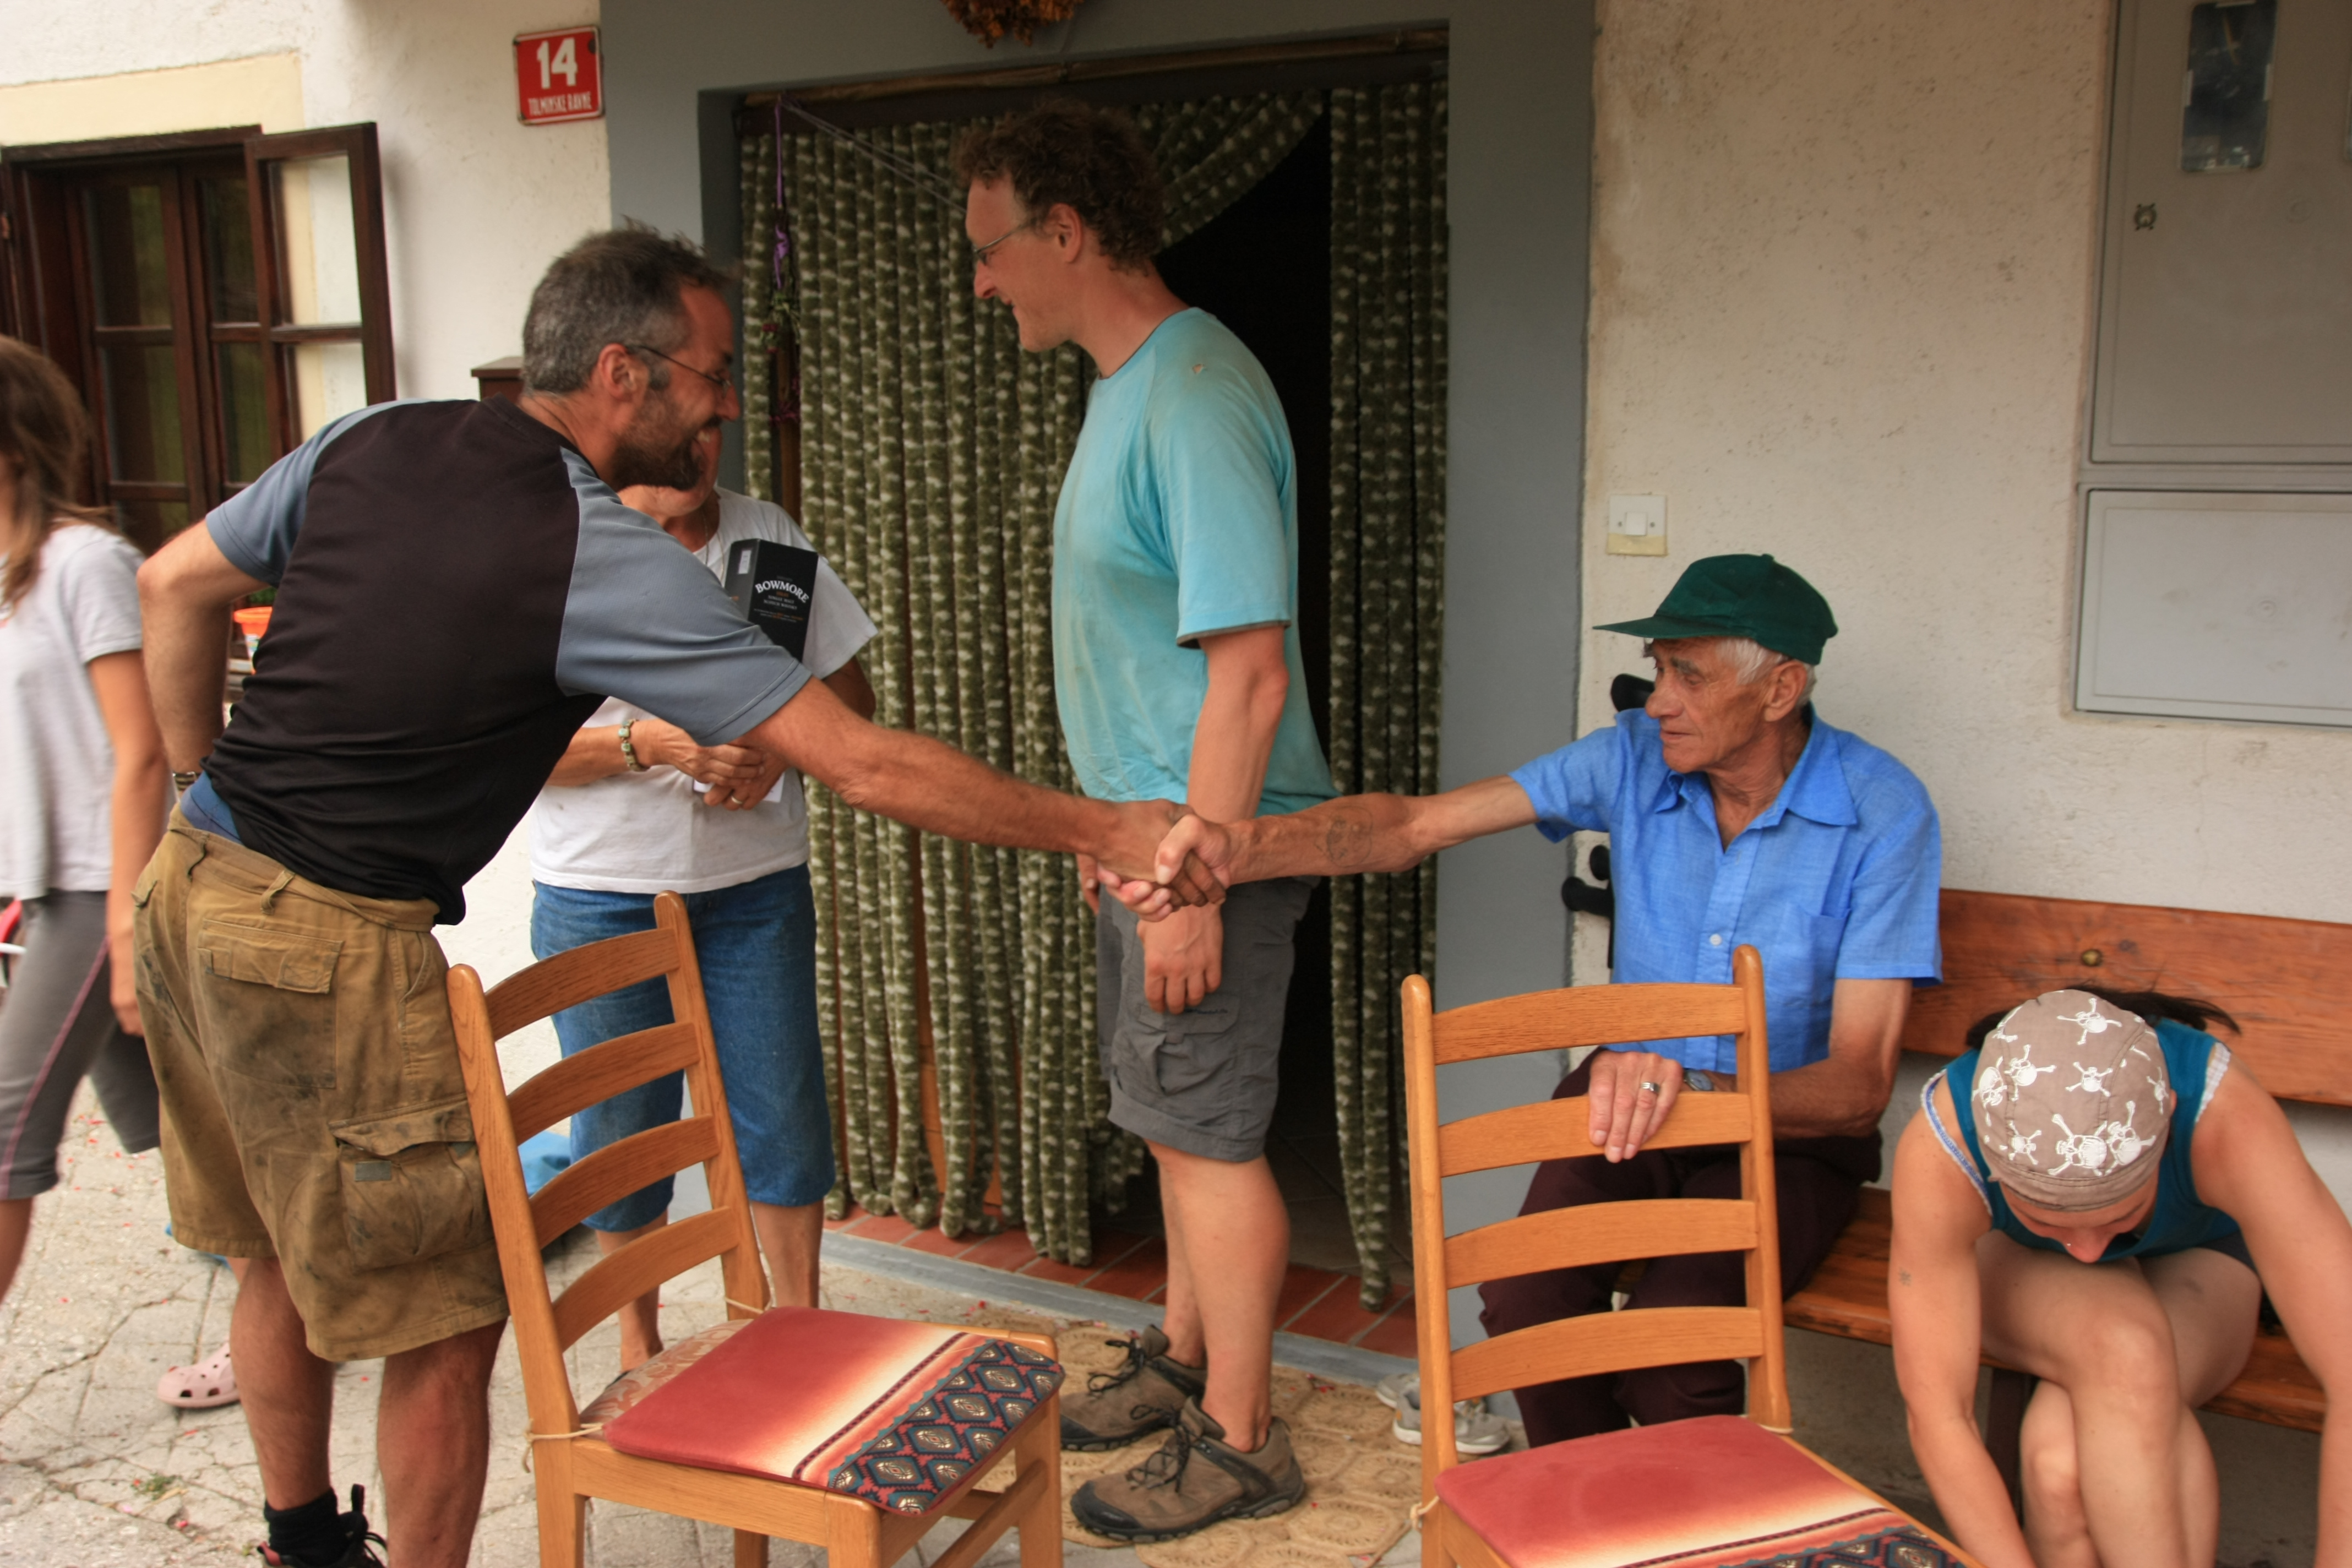
\includegraphics[width=\linewidth]{2012/press_release/2012-08-16-0703-GergelyAmbrus-IMG_2634--orig.jpg}} 
        \caption{} \label{marjan handshake}
    \end{subfigure}
    \caption{
    \textit{(a)} Andrej Fratnik being interviewed by Slovenian press. \pic{Jana Čarga}
    \textit{(b)} The JSPDT announce their success at Bar Kovačija in the centre of \passage[town]{Tolmin}. \pic{Jana Čarga}
    \textit{(c)} Tetley and Marjan shake hands in \passage[town]{Tolminske Ravne}. \pic{Gergely Ambrus}}
\end{figure*}
